\documentclass{article}
\usepackage{graphicx} % Required for inserting images
\usepackage{kotex}
\usepackage{subfigure}
\usepackage{caption}

\title{프로그래밍 언어 HW2}
\author{B811079 방병훈}
\date{20230427}

\begin{document}
\maketitle
\section{Section I. 실행 결과}
\begin{figure}[h]
    \centering
    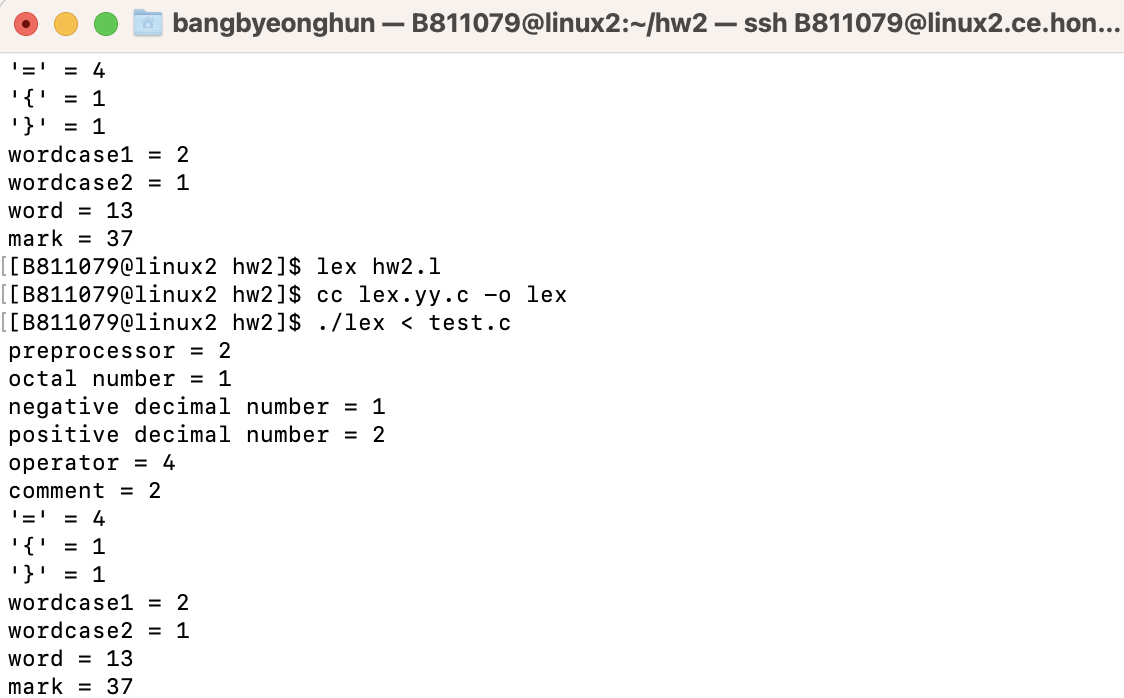
\includegraphics[width = 10cm]{run.png}
    \caption{실행결과}
    \label{fig:fig1}
\end{figure}
\section{Section II. 동작 방식 설명}
해당 코드는 정의절, 규칙절, 서브루틴절로 나뉘어있습니다. 주어진 파일을 시작부터 끝까지 의미 있는 단위로 분해해서 식별할 수 있는 루틴을 생성합니다. 최상단의 정의절에는 최종 프로그램에 포함하고자 하는 C프로그램의 내용을 삽입하고 출력을 위한 헤더와 분석한 코드의 수를 세는 변수가 포함됩니다.
규칙절에는 입력된 문자에서 매칭되는 문자열의 패턴과 해당 패턴이 나오면 수행할 동작으로 나뉩니다. 패턴은 정규표현식으로 구현했습니다. 먼저 작성된 규칙이 먼저 선택되므로 프로그램 안에서 먼저 수행되야할 코드들일수록 위에 배치했습니다. 마지막으로 서브루틴절에 출력 양식대로 출력을 하기 위해 print 문을 반복적으로 배치했습니다.
\section{Section III. 코드 설명}
\begin{figure}[h]
    \centering
    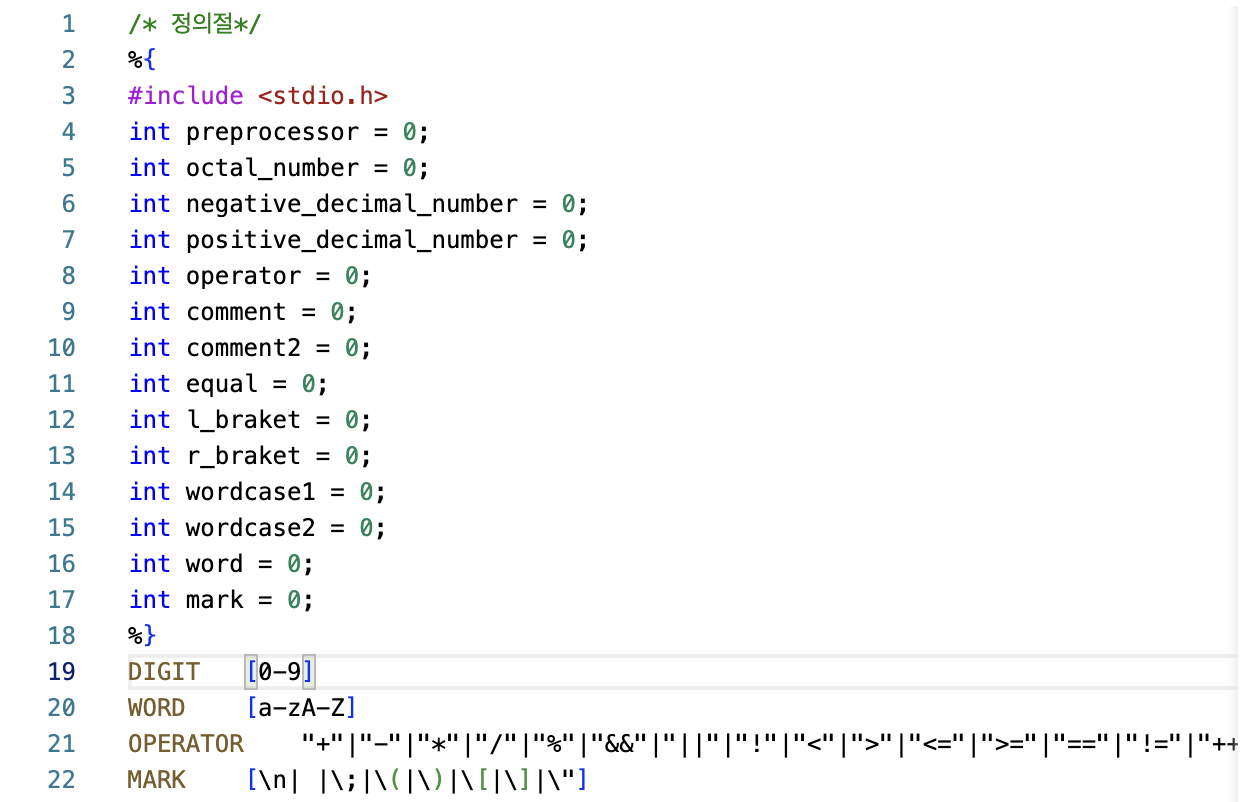
\includegraphics[width = 10cm]{code1.png}
    \caption{정의절}
    \label{fig:fig2}
\end{figure}
\begin{figure}[h]
    \centering
    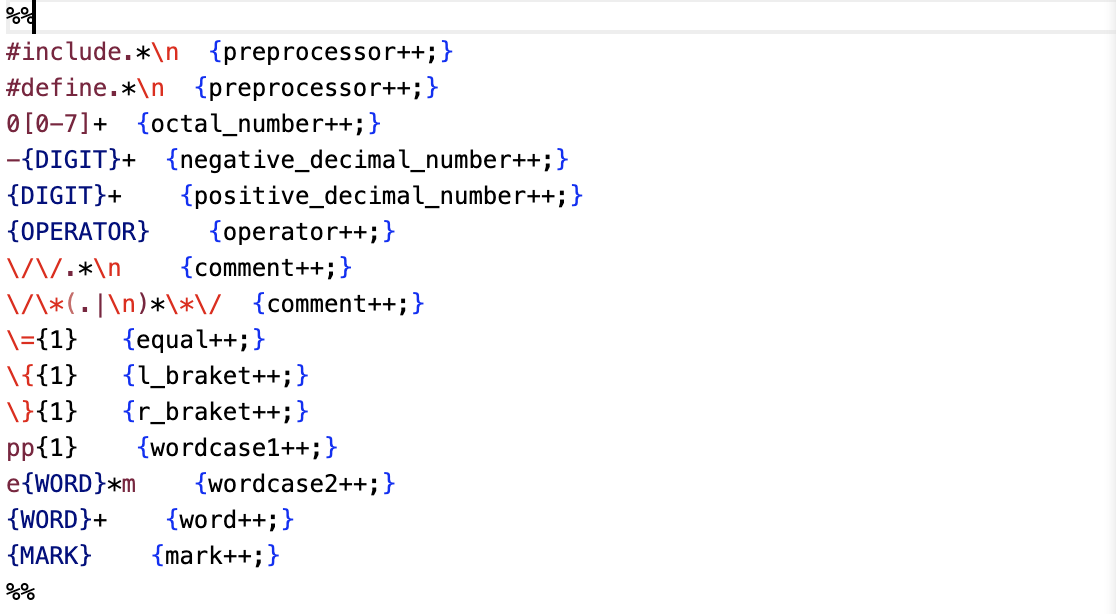
\includegraphics[width = 10cm]{code2.png}
    \caption{규칙절}
    \label{fig:fig3}
\end{figure}
\begin{figure}[ht]
    \centering
    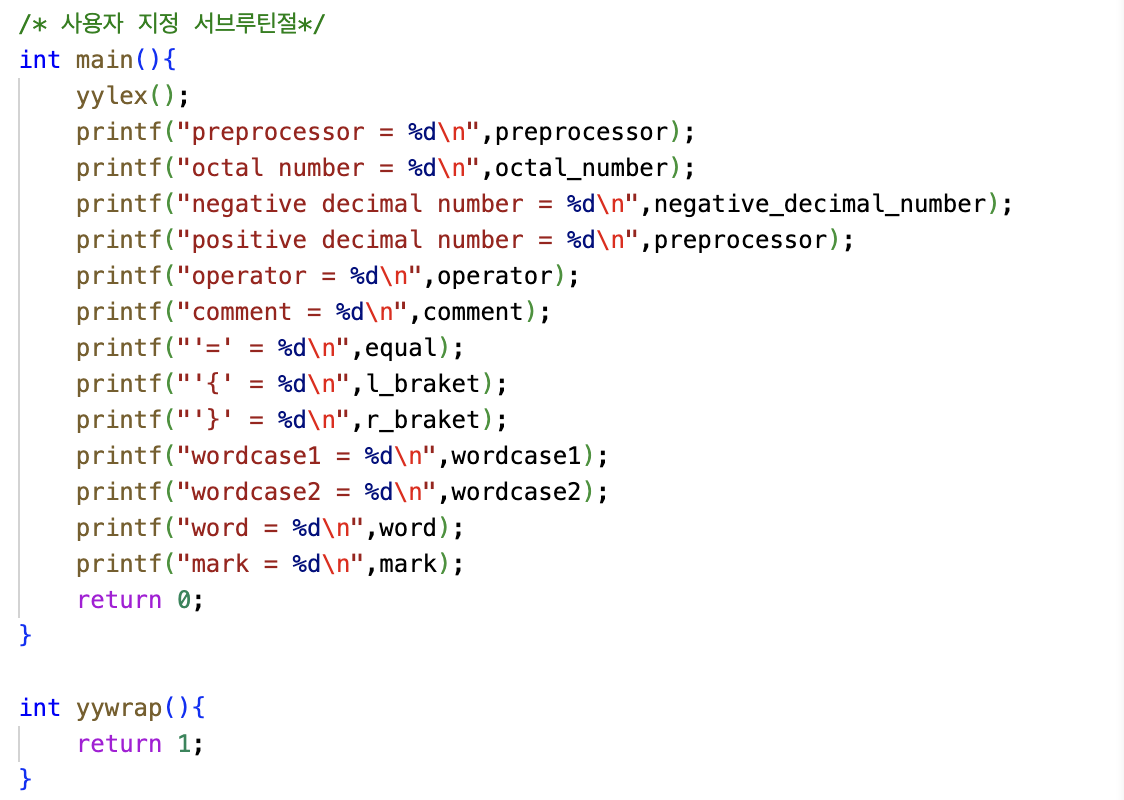
\includegraphics[width = 10cm]{code3.png}
    \caption{서브루틴절}
    \label{fig:fig4}
\end{figure}
\newpage
우선 정의절에 카운트에 필요한 변수들을 선언 및 초기화 했습니다. 그리고 코드가 직관적이고 코드를 작성할때 편의성을 위해서 DIGIT을 [0-9]로 WORD를 [a-zA-Z], OPERATOR는 연산자를, MARK는 나머지
카운트되지 않은 숫자들을 선언하였습니다. 처음에 preprocessor를 카운트하기 위해 \#include.*\\n을 했는데 \#include라는 문자열 뒤에 어떤 문자가 오던지 함께 카운트하고 개행문자도 추가적으로 세지지 않도록 뒤에 덧붙여서 작성했습니다. \#define도 마찬가지입니다. 8진수 숫자를 카운트하기위해 처음에 0으로 시작하는 특성을 살려 0[0-7]+로 했습니다. []안이 0-7인 이유는 팔진수이기 때문이고 자리수가 다양하므로 하나 혹은 그 이상을 뜻하는 +를 붙였습니다. 양의 정수를 셀때는 {DIGIT}+로 카운트 하였는데 양의 정수는 숫자0-9로만 표현되기 때문입니다. 자리수가 다양하므로 뒤에 +를 붙였습니다. 음의 정수도 앞에 -가 붙는다는 것 외에는 양의 정수와 마찬가지입니다. 제시된 조건에 맞는 연산자들은 모조리 OPERATOR로 선언해서 카운트했습니다. 그리고 주석의 경우도 //의 경우 뒤에 오는 문자열과 개행문자까지 포함해서 카운트해서 mark에서 오차가 발생하지 않도록 했습니다. 뒤에 오는 문자열은 .*를 통해 (.은 개행문자를 제외한 모든 문자) 어떤 문자가 오던 0번 이상 반복하는 *를 활용해서 카운트되도록 했습니다. 또한 /**/형태의 주석의 경우 문자열이 한문장일수도 있지만 여러줄일 경우도 있어 문자열과 그 사이에 포함된 개행문자까지 카운트할수 있도록 (.|\\n)*로 작성하였습니다. |를 활용해서 정규표현식을 작성하면 .이나 \\n중에서 고르기 때문에 개행문자까지 카운트 할 수 있습니다. =,\{,\} 세 가지 모두 1개만 카운트 해야하므로 역슬래시 뒤에 원하는 문자, 그리고 \{1\}를 작성해서 1개만 카운트하도록 했습니다. 앞선 경우와 동일하게 p가 두번만 반복되는 경우도 pp\{1\}로 표현했습니다. e로 시작해서 m으로 끝나는 단어는 앞에서 정의한 WORD를 활용해서 e\{WORD\}*m으로 작성했는데 시작은 e이고 중간에 알파벳문자열이 들어갈수 있게 하였고 그 뒤에 m을 붙여 m으로 끝나는 문자열만 추출하도록 했습니다. 남은 단어들은 알파벳으로 이뤄진 문자열이므로 \{WORD\}+로 알파벳이 1번 반복되면 카운트되도록 하였습니다. 앞에서 카운트되지 않은 문자들은 앞서 정의한 MARK를 통해 카운트되도록 하였습니다.
\end{document}
